\documentclass[11pt, oneside]{article}   	% use "amsart" instead of "article" for AMSLaTeX format
\usepackage{geometry}                		% See geometry.pdf to learn the layout options. There are lots.
\geometry{letterpaper}                   		% ... or a4paper or a5paper or ... 
%\geometry{landscape}                		% Activate for for rotated page geometry
%\usepackage[parfill]{parskip}    		% Activate to begin paragraphs with an empty line rather than an indent
\usepackage{graphicx}				% Use pdf, png, jpg, or eps� with pdflatex; use eps in DVI mode
								% TeX will automatically convert eps --> pdf in pdflatex		
\usepackage{amssymb}
\usepackage{amsmath}
\usepackage{parskip}
\usepackage{color}
\usepackage{hyperref}

\title{Functions of a complex variable:  Cauchy-Riemann equations}
%\author{The Author}
%\section{}
%\subsection*{}
\date{}							% Activate to display a given date or no date

\graphicspath{{/Users/telliott_admin/Dropbox/Tex/png/}}
% \begin{center} 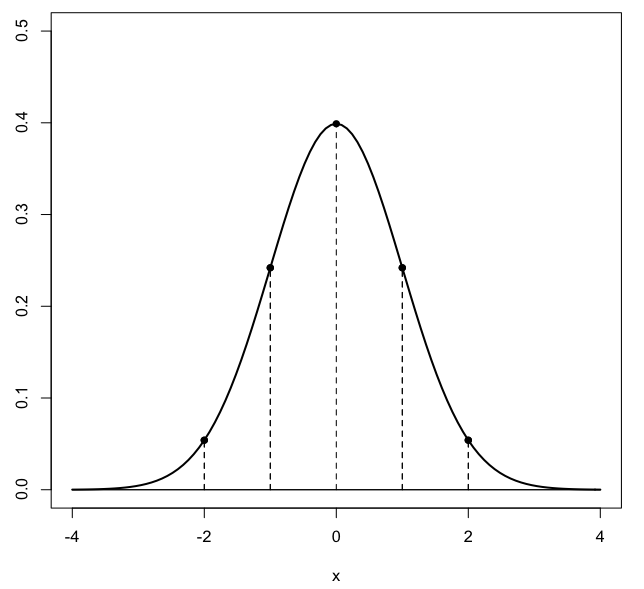
\includegraphics [scale=0.4] {gauss3.png} \end{center}
\begin{document}
\maketitle
\Large
Now we get to the point of these write-ups.  These are my notes on the calculus of complex functions.  The sources include the beginning of Chapter 6 in Shankar's Basic Training book, Boas Chapter 14, and Nahin's \emph{An imaginary tale: the story of} $\sqrt{-1}$, as well as a set of notes by Michael Alder that I found online (see sources).  

I have not worked through all of these, by any means.  I am just trying to solidify my understanding by writing things out in my own format, if not my own words entirely.

As Shankar says, just as we can associate with points on the $x$-axis a function $f(x)$, so we may associate with each point $(x,y)$ in the complex plane a function
\[ f(x,y) = u(x,y) + iv(x,y) \]
where $u(x,y)$ and $v(x,y)$ are real functions of two real variables i.e.
\[ f: \mathbb{R}^2 \rightarrow \mathbb{R}^1 \]
How to define continuity at a point for such a function?  Well, first the function must be defined \emph{at} the point.  And then the function must approach that value as the limit when approaching the point.

The new twist is that since we are in $\mathbb{R}^2$ there is an infinite number of directions from which we can approach, rather than just two as in $\mathbb{R}^1$.  

Example:  the function
\[ f(x,y) = \frac{x^2}{x^2 + y^2} \]
has some problems:  first, it is not defined at the origin $(0,0)$ but also, as we approach the origin along the $x$-axis and the $y$-axis we get different limiting values, namely
\[ f(x,0) = \frac{x^2}{x^2} = 1 \]
\[ f(0,y) = \frac{0}{y^2} = 0 \]

Rewriting it in polar coordinates ($x = r \cos \theta, r^2 = x^2 + y^2$):
\[ f(r,\theta) = \frac{r^2 \cos^2 \theta}{r^2} = \cos^2 \theta \]

Shankar says:  the function $f$ is generally a function of \emph{two} complex variables, $z$ and its complex conjugate:
\[ z = x + iy \]
\[ z* = x - iy \]
which can be written in terms of $x$ and $y$ as
\[ x = \frac{z + z*}{2} \]
\[ y = \frac{z - z*}{2i} \]
Generally, the value of $f$ depends on both $z$ and $z*$, but we will be very interested in functions which depend only on $z$ and not $z*$.  The reason for this is that only such functions have the property that the derivative at a point does not depend on the direction from which we approach that point.

Consider the function:
\[ f(x,y) = x^2 - y^2 \]
\[ = \frac{(z+z*)^2}{4} + \frac{(z-z*)^2}{4} \]
\[ = \frac{1}{4} \ [ \ z^2 + 2zz* + z*^2 + z^2 - 2zz* + z*^2 \ ] \]
\[ = \frac{z^2 + z*^2}{2} \]
This function is not a function only of $z$ but of both $z$ and $z*$.

We say that $f$ is an \emph{analytic} function of $z$ if it does not depend on $z*$.  Shankar says this means that "$x$ and $y$ enter $f$ \emph{only} in the combination $x + iy$".

The famous Cauchy-Riemann Equations (CRE) are true for $f \iff f$ is an analytic function of $z$.  

For:
\[ f(x,y) = u(x,y) + iv(x,y) \]
The CRE conditions are:
\[ u_x = v_y \]
\[ u_y = -v_x \]
We'll talk about derivations below but let's just try them out.

Consider:
\[ f(x,y) = x^2 - y^2 + i2xy \]
CRE requires
\[ u_x = 2x \stackrel{?}{=}  v_y = 2x \]
\[ v_x = 2y \stackrel{?}{=} - u_y = 2y \]
The function is analytic.  As Shankar says, this is expected because:
\[ x^2 - y^2 + 2ixy = (x + iy)(x + iy) = z^2 \]

Consider:
\[ f(x,y) = \cos y - i \sin y \]
CRE requires:
\[ u_x = 0 \stackrel{?}{=} v_y = - \cos y \]
\[ v_x = 0 \stackrel{?}{=}  -u_y = - \sin y \]
This is "impossible" since there is no $y$ that satisfies both of the conditions.  And it's not surprising since
\[ y = \frac{z - z*}{2i} \]

Consider:
\[ f(x,y) = x^2 + y^2 \]
CRE requires:
\[ u_x = 2x \stackrel{?}{=}  v_y = 2y \]
\[ u_y = 0 \stackrel{?}{=}  -v_x \]
CRE are only satisfied if $x=y$.  Also not surprising since
\[ x^2 + y^2 = zz* \]

Consider:
\[ f(x,y) = x^2 - y^2 \]
CRE requires:
\[ u_x = 2x \stackrel{?}{=} v_y = -2y \]
which is true if $x = y$.
\[ u_y = 0 \stackrel{?}{=} -v_x = 0 \]
But "no importance is given to functions which obey the CRE only at isolated points or on lines."

Consider:
\[ f(x,y) = e^x \cos y + i e^x \sin y \]
CRE requires:
\[ u_x = e^x \cos y \stackrel{?}{=} v_y = e^x \cos y \]
\[ u_y = -e^x \sin y \stackrel{?}{=} -v_x = - \sin y e^x \]
Both are true, so this one does satisfy CRE.

Shankar doesn't mention it here but the last function is special, it is $f(z) = e^z$:
\[ e^x \cos y + i e^x \sin y \]
\[ = e^x (\cos y + i \sin y) \]
\[ = e^x e^{iy} \]
\[ = e^{x + iy} \]
\[ = e^z \]
and we did this one in the previous section.

For functions of interest, it may often be true that CRE fails at particular points called \emph{singularities}.

Consider:
\[ f(x,y) = \frac{1}{z} = \frac{z*}{zz*} = \frac{x-iy}{x^2 + y^2} \]
We need:
\[ u_x = \frac{d}{dx} \ \frac{x}{x^2 + y^2} = \frac{x^2 + y^2 - 2x^2}{(x^2 + y^2)^2}  = \frac{y^2 - x^2}{(x^2 + y^2)^2} \]
\[ v_y = \frac{d}{dy} \ (-\frac{y}{x^2 + y^2} ) = - \frac{x^2 - y^2}{(x^2 + y^2)^2} = u_x \]
\[ u_y =  0 = v_x \]
But the function blows up at the origin.  This described by saying it has a pole at the origin.
The function
\[ f(z) = \frac{c}{z} \]
where $c$ is a constant, also blows up at the origin.  We say that the \emph{residue} of the pole at the origin is $c$.

For a function to be analytic it must be true that
\[ f_x = - i f_y \]
(see below) where
\[ f_x = \frac{\partial f}{\partial x} \]
\[ f_y = \frac{\partial f}{\partial y} \]

Thus
\[ f_x = u_x + iv_x \]
\[ f_y = u_y + iv_y \]
\[ -i f_y = -i(u_y + iv_y) = v_y - iu_y \]
Since both real and imaginary parts must be equal, we obtain the CRE.

\subsection*{Proof of CRE}

Write:
\[ z = x + iy \]
Clearly,
\[ \frac{\partial z}{\partial x} = 1 \]
\[ \frac{\partial z}{\partial y} = i \]
Now,
\[ w = f(z) \]
\[ = u(x,y) + i \ v(x,y) \]
where $u$ and $v$ are real functions over $\mathbb{R}^2$.

Recalling the chain rule
\[ w = u(x,y) + i \ v(x,y) \]
\[ \frac{\partial w}{\partial x} = \frac{dw}{dz} \ \frac{\partial z}{\partial x} \]
\[ =  \frac{dw}{dz} \]
(by the result immediately above, that $\partial z/\partial x = 1$).
Similarly
\[ \frac{\partial w}{\partial y} = \frac{dw}{dz} \ \frac{\partial z}{\partial y} \]
\[ =  i \frac{dw}{dz} \]
Hence we can equate the two expressions for $dw/dz$:
\[ \frac{dw}{dz} = \frac{\partial w}{\partial x} = -i \frac{\partial w}{\partial y} \]

Now if we actually compute the partials and plug them in to the last equation, we obtain:
\[ \frac{\partial w}{\partial x} = u_x + i v_x \]
\[ \frac{\partial w}{\partial y} = u_y + i v_y \]
\[ u_x + i v_x = -i (u_y + i v_y) = v_y - i u_y \]
Both the real and the imaginary parts must be equal:
\[ u_x = v_y \]
\[ v_x = - u_y \]
These are the CRE.

It is worth taking a breath for a moment and repeating what we just said:  the derivative of an analytic (that is, differentiable) complex function $z$ is
\[ \frac{df}{dz} = \frac{\partial f}{\partial x} = - i \frac{\partial f}{\partial y} \]
\[ = u_x + i v_x \]
\[ = -i (u_y + i v_y) \]
\[ = v_y - i u_y\] 

\subsection*{a second derivation}
Because this is all still quite new it may be useful to work through an apparently different derivation of the CRE, as presented in Nahin.  Consider how to define the derivative of a complex function.  Suppose we define:
\[ \frac{df}{dz} = f'(z_0) \]
\[ = \lim_{\Delta z \rightarrow 0} f(z_0 + \Delta z) - f(z_0) / \Delta z \]
Now 
\[ z = f(x,y) = x + iy \]
So
\[ f'(z_0) = \lim_{\Delta x, \Delta y \rightarrow 0} f(x_0 + \Delta x, y_0 + \Delta y) - f(x_0,y_0) / \Delta x + i \Delta y \]
And now we insist that the value of the derivative should be independent of the direction of approach to the origin.  So, out of all the possible approaches, come along the $x$-axis or along the $y$-axis.  In the first case, $\Delta y = 0$ and we have
\[ f'(z_0) = \lim_{\Delta x \rightarrow 0} f(x_0 + \Delta x, y_0) - f(x_0,y_0) / \Delta x \]
Expand in $u$ and $v$
\[ = \lim_{\Delta x \rightarrow 0} u(x_0 + \Delta x, y_0) + iv(x_0 + \Delta x, y_0) - u(x_0,y_0) - ivu(x_0,y_0) / \Delta x \]
\[ = \lim_{\Delta x \rightarrow 0} u(x_0 + \Delta x, y_0) - u(x_0,y_0) + iv(x_0 + \Delta x, y_0) - ivu(x_0,y_0) / \Delta x \]
\[ = u_x + i v_x \]
Similarly, approaching along the $y$-axis ($\Delta x = 0$):
\[ f'(z_0) = \lim_{\Delta y \rightarrow 0} f(x_0, y_0 + \Delta y) - f(x_0,y_0) / i\Delta y \]
Expand in $u$ and $v$
\[ = \lim_{\Delta y \rightarrow 0} u(x_0, y_0 + \Delta y) + iv(x_0, y_0 + \Delta y) - u(x_0,y_0) - ivu(x_0,y_0) / i \Delta y \]
\[ = \lim_{\Delta y \rightarrow 0} u(x_0, y_0 + \Delta y) - u(x_0,y_0) + iv(x_0, y_0 + \Delta y) - ivu(x_0,y_0) / i \Delta y \]
\[ = \frac{1}{i} (u_y + iv_y) \]
\[ = v_y - i u_y \]
Insisting that these two values for the derivative must be equal:
\[ u_x + i v_x = v_y - i u_y \]
Since both real and imaginary parts must be equal, we have the CRE.

A third, very simple proof is given in Alder:

Suppose $f: C \rightarrow C$ is a function, taking $x+iy$ to $u(x,y) + iv(x,y)$, then the derivative is a matrix of partial derivatives:
\[
\begin{matrix}
u_x &  u_y \\
v_x & v_y
\end{matrix}
\]
.. the above matrix is the two dimensional version of the slope of the tangent line in dimension one.  It gives the linear part (corresponding to the slope) of the affine map which best approximates $f$ at each point.

.. if $f$ is differentiable in the \emph{complex} sense, this must be just a linear complex map, i.e. it multiplies by some complex number.  So the matrix must be in our set of complex numbers.  In other words, for every value of $x$ it looks like
\[
\begin{matrix}
a & -b \\
b & a
\end{matrix}
\]
for some real numbers $a,b$, which change with $x$.

Of course, this constraint leads directly to the CRE.

Sources:

[1] Alder.  \emph{An Introduction to Complex Analysis for Engineers}.

\url{http://www.eee.metu.edu.tr/~ccandan/EE202_summer2004/solutions/An%20Introduction%20to%20Complex%20Analysis%20for%20Engineers%20-%20Michael%20Alder.pdf}

[2] Boas. \emph{Mathematical methods in the Physical Sciences}.

[3] HELM workbooks, No. 26.

\url{http://www.personal.soton.ac.uk/jav/soton/HELM/helm_workbooks.html}

[4] Marsden and Hoffman.  \emph{Basic Complex Analysis}

\url{http://www.matem.unam.mx/ernesto/LIBROS/AC/Marsden-Jerrold-Michael%20J.%20Hoffman-Basic%20Complex%20Analysis.pdf}

[5] Nahin.  \emph{An imaginary tale:  the story of $\sqrt{-1}$}

[6] Shankar.  \emph{Basic Training in Mathematics}.

\end{document}  